\section{Diseño y resolución}

En este apartado vamos a pasar a explicar los detalles del desarrollo del proyecto. Como se ha dicho, el proyecto consiste en realizar un sistema capaz de seguir los movimientos del balón y las jugadoras de un partido de volleyball mediante imágenes proporcionadas por una cámara en vista cenital.

El seguimiento se puede realizar por \textit{tracking}, sustracción de fondo, o bien un sistema que aúne ambas cosas para una mayor robustez.

Una vez resuelta la parte del seguimiento, el siguiente objetivo sería registrar las posiciones detectadas a un fichero de salida en formato CSV, mediante el cual se puedan hacer análisis de distintas métricas del juego.

El desarrollo se va a centrar, como he ido aclarando, en una aplicación en Python utilizando OpenCV y PyQt para la parte de interfaz gráfica. De cara a la construcción del sistema, la estrategia a seguir es desarrollar separadamente sus partes y posteriormente implementarlas para que funcionen de manera conjunta.

A continuación detallaré estas partes y cómo se ha resuelto su implementación. Las partes principales del sistema son: sustracción de fondo, seguimiento (\textit{tracking}), interfaz gráfica y métodos de consistencia temporal???

\subsection{Sustracción de fondo}
Teniendo en cuenta que la cámara es fija y cenital, y por tanto el fondo siempre va a ser exactamente el mismo, una primera aproximación ingenua a este problema podría ser tan simple como realizar una diferencia entre los frames del video.

Por desgracia, las condiciones de iluminación no siempre van a ser totalmente iguales, lo cual va a dificultar en gran medida la detección de objetos usando este método. Además, no siempre vamos a tener disponible una imagen limpia del campo en un video, por lo que es complicado realizar un modelo del campo para las diferentes condiciones de iluminación a lo largo de un día.

Una vez hemos podido ver que esta manera de proceder no es todo lo viable que cabría desear, podemos empezar a plantearnos otras opciones a nuestra disposición. OpenCV proporciona distintos algoritmos de sustracción de fondo, los cuales podemos aprovechar y comparar para ver cuál es más apropiado para nuestro propósito.

\begin{figure}
    \centering
    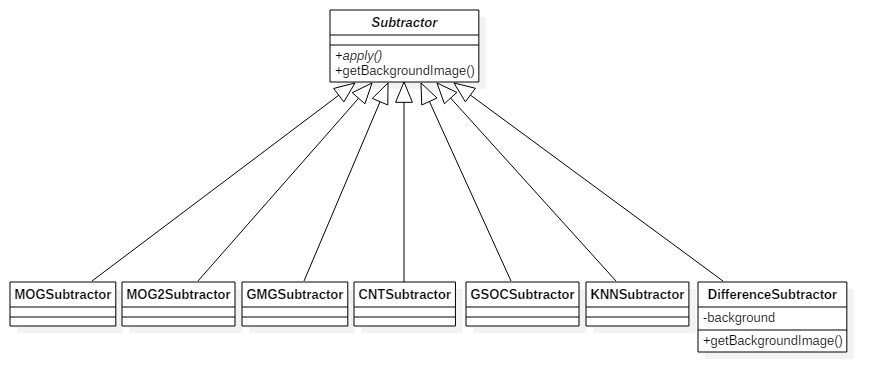
\includegraphics[width=0.9\textwidth]{images/subtractors}
    \caption{Estructura de clases de los sustractores de fondo}
    \label{fig:subtractors}
\end{figure}

Para facilitar el uso de estos algoritmos, se ha hecho uso de la programación orientada a objetos que nos ofrece Python. Se ha creado una clase abstracta llamada Subtractor de la cual heredan todas las clases que hagan uso de los algoritmos de OpenCV así como el de diferencia de frames. Dicha clase proporciona una interfaz común a todas las clases, que hará mas sencillo el uso de ellas. La estructura resultante puede verse en la figura \ref{fig:subtractors}.

El funcionamiento interno de las clases resultantes, como se ha dicho, corresponde a las propias implementaciones de OpenCV. Pasaré a explicar los fundamentos teóricos de cada uno de estos algoritmos

\subsubsection*{MOG}
MOG, mezcla de gaussianas (\textit{Mixture of Gaussians}), fue descrito en  \cite{KaewTraKulPong2002} 

\subsubsection*{MOG2}
MOG2 es un algoritmo propuesto en los trabajos \cite{art:Zivkovic1} y \cite{art:Zivkovic2} de Z. Zivkovic. Es una mejora sobre la versión anterior, MOG

\subsection{Seguimiento}

\subsection{Interfaz gráfica}


